\documentclass[8.01x]{subfiles}
\begin{document}

\chapter{Week 12: Homework 9}

\section{Problem 1: Crane}

``A crane is configured as below, with the beam suspended at two points $\ell_1$ and $\ell_2$ by each end of a cable passing over a frictionless pulley. The two ends of the cable each make an angle $\theta$ with the beam. A counterbalance object C with mass $m_C$ is fixed at one end of the beam. A balance object B of mass $m_B$ is attached to the beam and can move horizontally in order to maintain static equilibrium. The crane lifts an object A with mass $m_A$ at a distance $y$ from the counterbalance. For simplicity, assume the pulley, beam and cable to be massless.

\begin{center}
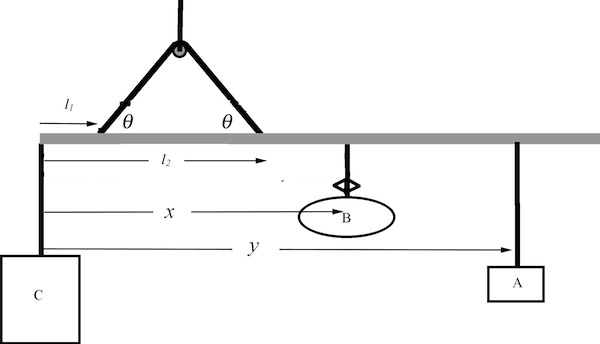
\includegraphics[scale=2.5]{Graphics/h9p1} % Image is 150 dpi, hmm.
\end{center}

(a) What is the tension in the cable that runs over the pulley? Express your answer in terms of $m_A$, $m_B$, $m_C$, $\theta$ and acceleration due to gravity $g$.\\
(b) At what horizontal position, $x$, should one put the balance object B such that the crane doesn't tilt? Express your answer in terms of $m_A$, $m_B$, $m_C$, $\ell_1$, $\ell_2$ and $y$.''

Let's first consider the vertical forces on the beam. We have three weights, balanced by the same tension in two places; the tensions need to be decomposed, though. If the angle was 90 degrees, the vertical component of the tension would clearly be at a maximum, so we need a sine in there (which drawing it out and doing the trigonometry confirms):

\begin{equation}
g(m_A + m_B + m_C) = 2 T \sin \theta
\end{equation}

We only need to divide both sides by $2 \sin \theta$, and we have the answer to part (a):

\begin{equation}
\frac{g(m_A + m_B + m_C)}{2 \sin \theta} = T
\end{equation}

For part (b), we need to consider the torque on the system. We can calculate torques relative to any point of our choosing, but what point would make things the easiest? If we choose $x = 0$, the torque due to mass C disappears. The same argument holds for other points and other masses. Just below the cable, between the two tensions, the torques due to both tensions cancel out.

Because the answer doesn't allow $\theta$ and doesn't allow $g$, we should choose the point where the tensions cause no torque. That way, all disallowed variables should either not enter the equation ($\theta$) or cancel ($g$).\\
I will call that point $\displaystyle b = \ell_1 + (\ell_2 - \ell_1)/2 = \frac{\ell_1 + \ell_2}{2}$, to reduce clutter in the torque equation. I use out of the screen as the positive direction.

\begin{equation}
\tau_b = b g m_C - (x - b) g m_B - (y - b) g m_A
\end{equation}

This must be equal to zero. $g$ cancels, as hoped for/expected.

\begin{align}
0 &= b m_C - (x - b) m_B - (y - b) m_A\\
x m_B &= b m_C + b m_B - y m_A + b m_A\\
x &= \frac{b(m_C + m_B + m_A) - y m_A}{m_B}\\
x &= \frac{\frac{\ell_1 + \ell_2}{2} (m_C + m_B + m_A) - y m_A}{m_B}
\end{align}

We would, in the end, find the same answer if we calculated the torque relative to any other point (the torque relative to any point is equal in static equilibrium; the book shows how).

\section{Problem 2: Steel beam and cable}

``A uniform steel beam of mass $m_1 = \SI{150.0}{kg}$ is held up by a steel cable that is connected to the beam a distance $L = 5.0$ m from the wall, at an angle $\theta = \ang{35.0}$ as shown in the sketch. The beam is bolted to the wall with an unknown force $\vec{F}$ exerted by the wall on the beam. An object of mass $m_2 =  \SI{60.0}{kg}$ resting on top of the beam, is placed a distance $d = 2.0$ m from the wall. For simplicity, assume the steel cable to be massless. Use $g = \SI{9.8}{m/s^2}$ for the gravitational acceleration.

\begin{center}
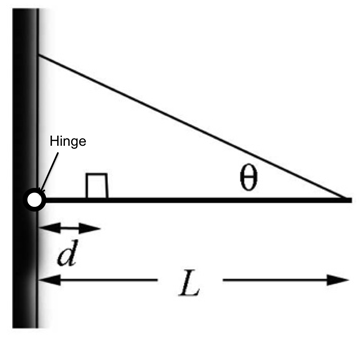
\includegraphics[scale=1.15]{Graphics/h9p2}
\end{center}

(a) Find the tension (in Newton) in the cable. Start by drawing a free-body diagram for the beam, then find equations for static equilibrium for the beam (this will involve force equations and torque relations).
(b) Find the horizontal and vertical components of the force (in Newton) that the wall exerts on the beam.''

Okay. There are four forces on the beam (with 1 or 2 components each): normal force (2 components) at the hinge, gravity acting purely downwards at the center of mass ($L/2$), gravity acting purely downwards at $d$ and the tension (2 components) at the end of the beam.

The tension clearly acts upwards and inwards, so the normal force must act outwards (towards the right), as they are the only two horizontal forces. Whether the normal force acts upwards or downwards I don't know however, since there is also gravity in the mix. I will guess that it acts upwards, and so if it turns out negative, I guessed wrong.

For the tensions, we have

\begin{align}
T_x &= -T \cos \theta\\
T_y &= T \sin \theta
\end{align}

using a coordinate system where $+x$ is towards the right. We can now calculate the sum the forces in the vertical direction to zero:

\begin{equation}
N_y + T \sin \theta - g(m_1 + m_2) = 0
\end{equation}

One equation, two unknowns. Next, we can consider torque. The net torque relative to any point must be zero. If we choose the point right at the hinge, the unknown normal force doesn't cause a torque, so we get

\begin{equation}
g\left(\frac{L}{2} m_1 + d m_2\right) - L T \sin \theta = 0
\end{equation}

The horizontal forces also cannot cause at torque relative to this point. We now have two equations and two unknowns, though we also need to find $N_x$ later on. That turns out to be trivial, however, so let's begin with $T$ and $N_y$.

Note that $T$ is the only unknown in this second equation, so we start by finding that:

\begin{align}
g\left(\frac{L}{2} m_1 + d m_2\right) &= L T \sin \theta\\
\frac{g\left(\frac{L}{2} m_1 + d m_2\right)}{L \sin \theta} &= T
\end{align}

For the given values, $T = 1691.5$ newton. We can then find $N_y$ by solving the previous equation for that, and sticking in this value of $T$.

\begin{align}
N_y &= g(m_1 + m_2) - T \sin \theta\\
N_y &= g(m_1 + m_2) - \frac{g\left(\frac{L}{2} m_1 + d m_2\right)}{L}
\end{align}

For the given values, $N_y = 1087.8$ newton.

As for $N_x$, it and $T_x$ are the only two horizontal forces. Therefore, they must be equal in magnitude, and so $N_x = T \cos \theta = 1385.6$ N.

\section{Problem 3: Person on ladder}

``A person of mass $m_2 = 85.0$ kg is standing on a rung, one third of the way up a ladder of length $d = 4.0$ m. The mass of the ladder is $m_1 = 15.0$ kg, uniformly distributed. The ladder is initially inclined at an angle $\theta = \ang{40.0}$ with respect to the horizontal. Assume that there is no friction between the ladder and the wall but that there is friction between the base of the ladder and the floor with a coefficient of static friction $\mu_s$.

\begin{center}
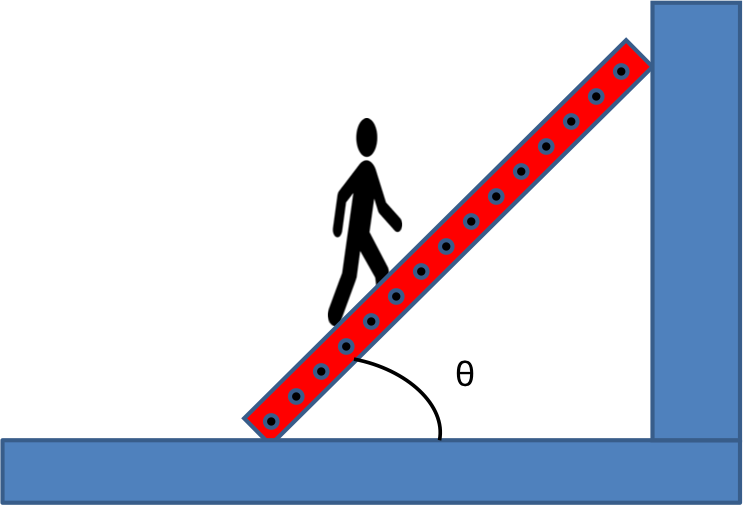
\includegraphics[scale=0.8]{Graphics/h9p3}
\end{center}

Start this problem by drawing a free-body force diagrams showing all the forces acting on the person and the ladder. Indicating a choice of unit vectors on your free-body diagrams may be helpful.

(a) Using the equations of static equilibrium for both forces and torque, find expressions for the normal and horizontal components of the contact force between the ladder and the floor, and the normal force between the ladder and the wall. Consider carefully which point to use for computing the torques. Determine the magnitude of the frictional force (in N) between the base of the ladder and the floor below.\\
(b) Find the magnitude for the minimum coefficient of friction between the ladder and the floor so that the person and ladder does not slip.\\
(c) Find the magnitude $C_{ladder,ground}$ (in N) of the contact force that the floor exerts on the ladder. Remember, the contact force is the vector sum of the normal force and friction.\\
Find the direction of the contact force that the floor exerts on the ladder. i.e. determine the angle $\alpha$ (in radians) that the contact force makes with the horizontal to indicate the direction.''

We could probably use the equations from lecture most of the way, but I will re-derive everything here anyway.

The vertical forces consist of the normal force where the ladder touches the ground (I call this point Q), gravity due to the person at $d/3$ along the length, and gravity at the ladder's center of mass $d/2$ along the length. Therefore,

\begin{equation}
N_Q = g(m_1 + m_2)
\end{equation}

In the horizontal direction, we have the normal force from the wall (point P) $N_P$ towards the left, and a frictional force $f_s \le \mu N_Q$ at point Q towards the right (since the ladder wants to slip towards the left).\\
This gives us, just at the edge of slipping ($f_s = \mu_s N_Q$, i.e. the maximum friction possible):

\begin{equation}
N_P = f_s = \mu_s N_Q
\end{equation}

Next, we can consider the torque. I will calculate them relative to point Q, so that two out of the five forces/force components ``disappear'' (they can't cause torque through that point). I will use into the screen (clockwise rotation) as positive, since that is how the ladder wants to rotate.

Now, these cross products depend on the angle, but the angle between the position vector from Q to where gravity acts, and the gravitational force vector, is not $\theta$. Indeed, it's easy to see that if $\theta = 0$, the angle between them would be 90 degrees. The relevant angle is $\ang{90} - \theta$, so that is what we need for the cross products; also, $\sin(\ang{90} - \theta) = \cos(\theta)$.\\
$\theta$ is the relevant angle for the normal force at P, however, so that one remains a sine.\\
Alternatively, we can try to find the perpendicular distance of either vector, and multiply that by the full magnitude of the other, which is the same thing.

\begin{equation}
\tau_Q = \frac{d}{3} m_2 g \cos \theta + \frac{d}{2} m_1 g \cos \theta - d N_P \sin \theta
\end{equation}

This needs to be equal to zero. We can set it equal to zero, solve for $N_P$ (which we earlier said was equal to $f_s$ in magnitude) and find the answer for part (a):

\begin{align}
0 &= \frac{d}{3} m_2 g \cos \theta + \frac{d}{2} m_1 g \cos \theta - d N_P \sin \theta\\
N_P &= \frac{\frac{d}{3} m_2 g \cos \theta + \frac{d}{2} m_1 g \cos \theta}{d \sin \theta}\\
f_s = N_P &= g \cot \theta \left(\frac{m_2}{3} + \frac{m_1}{2}\right)
\end{align}

(Since $f_s = N_P$.)\\
All variables above are known, so we can calculate $f_s = 418.5$ N.

Next, we need to find $\mu_s$. $f_s = \mu_s N_Q$, and we know $N_Q$ to be the sum of the two weights, $g(m_1 + m_2)$.

\begin{align}
\mu_s &= \frac{1}{g(m_1 + m_2)} g \cot \theta \left(\frac{m_2}{3} + \frac{m_1}{2}\right)\\
\mu_s &= \frac{1}{m_1 + m_2} \cot \theta \left(\frac{m_2}{3} + \frac{m_1}{2}\right)\\
\mu_s &= \frac{cot \theta(2 m_2 + 3 m_1)}{6(m_1 + m_2)}
\end{align}

In terms of numbers, $\mu_s \ge 0.427$ will meet this condition, so that there is no sliding.

Next, they want the magnitude and angle of the contact force. $N_Q = g(m_1 + m_2) = 980$ N, and $f_s = 418.5 N$. In terms of unit vectors,

\begin{equation}
C_{ladder,ground} = f_s \hat{x} + N_Q \hat{y}
\end{equation}

The magnitude of this vector is $C_{ladder,ground} = \sqrt{418.5^2 + 980^2} = 1065.6$ N. The angle $\alpha$ must be less than 90 degrees, or the friction would point towards the left. It is found as $\displaystyle \alpha = \arctan \frac{N_Q}{f_s}$, which is about 1.167 radians, or 66.88 degrees.

\section{Problem 4: Static equilibrium arm}

``You are holding a ball of mass $m_2$ in your hand. In this problem you will solve for the upward force $\vec{T}$ that the tendon of your biceps muscle exerts to keep the forearm horizontal and the downward force $\vec{F}$ that the upper arm exerts on the forearm at the elbow joint. Assume the outstretched arm has a mass of $m_1$, the center of mass of the outstretched arm is a distance $s$ from the elbow, the tendon attaches to the bone a distance $d$ from the elbow, and the ball is a distance $2s$ from the elbow. (Taking $\vec{T}$ to be upward and $\vec{F}$ to be downward, with no horizontal components, indicates that this is a simplified model.)\\
A schematic representation of this situation is shown below:

\begin{center}
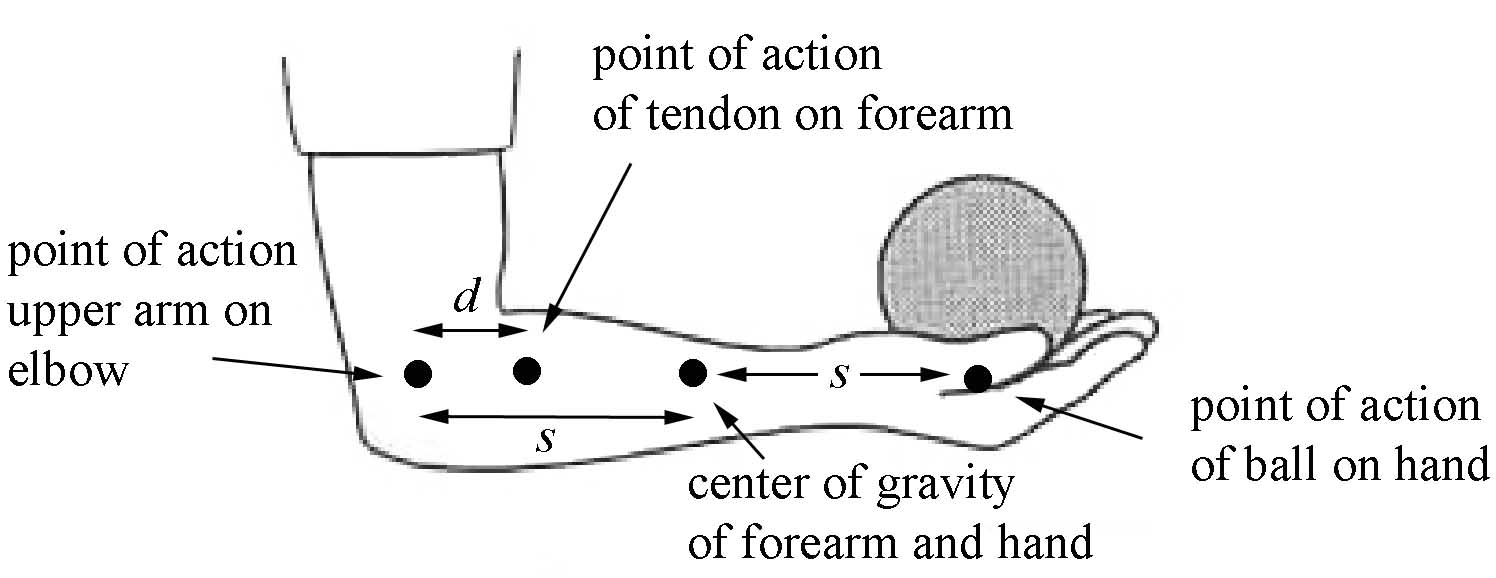
\includegraphics[scale=1.0]{Graphics/h9p4_1}
\end{center}

Hint: The forces can be modeled as shown in the following Free Body Diagram:

\begin{center}
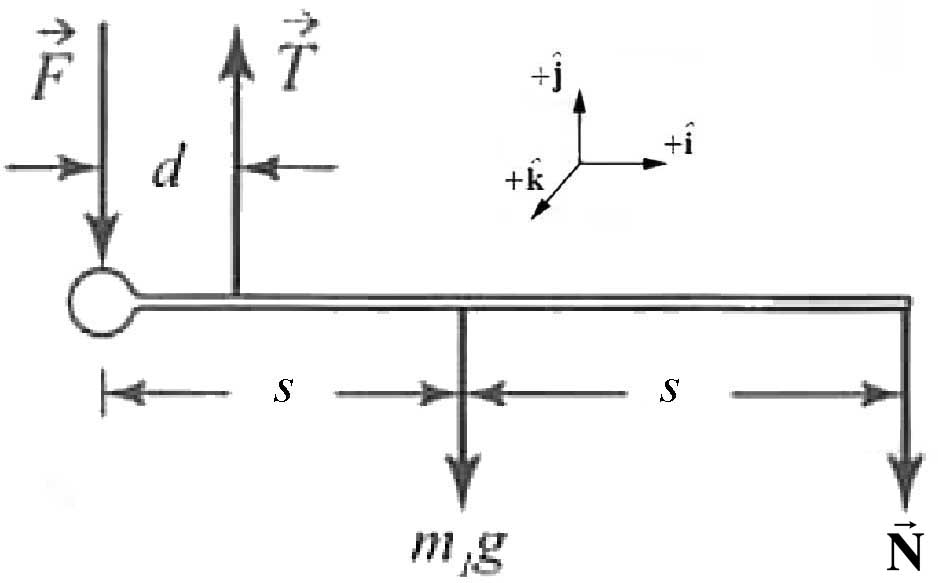
\includegraphics[scale=1.0]{Graphics/h9p4_2}
\end{center}

(a) What is the magnitude of the tension $T \equiv |\vec{T}|$ in the tendon? Express your answer in terms of $s$, $m_1$, $m_2$, $d$ and $g$ as needed.\\
(b) What is the magnitude of the force that the upper arm exerts on the forearm at the elbow joint? Express your answer in terms of $s$, $m_1$, $m_2$, $d$ and $g$ as needed.''

The problem description certainly sounds complex, but given the diagram and even a free body diagram, this should be one of the easier problems of the week. I choose a coordinate system with $x = 0$ and $y = 0$ at the elbow joint, with $+x$ to the right and $+y$ upwards (which I just noticed is marked in the free body diagram).

We need a net force of zero in the vertical direction, which gives us our first equation (equating upwards and downwards forces):

\begin{equation}
T = F + m_1 g + m_2 g
\end{equation}

where $m_2 g$ is equal in magnitude to the normal force from the hand to the ball.

Next, the torques must be zero, relative to any point of our choosing. I choose the center of the coordinate system, so that $F$ causes no torque. Downwards forces then cause a counterclockwise (into the screen) torque, which I denote as positive.

\begin{equation}
\tau = - d T + s m_1 g + 2 s m_2 g
\end{equation}

This must be equal to zero; we can set it as such and solve for $T$:

\begin{align}
0 &= - d T + s g ( m_1 + 2 m_2)\\
T &= \frac{s g (m_1 + 2 m_2)}{d}
\end{align}

This answers part (a); for part (b), we solve the force equation for $F$ and substitute in $T$.

\begin{align}
F &= T - g(m_1 + m_2)\\
F &= \frac{s g (m_1 + 2 m_2)}{d} - g(m_1 + m_2)
\end{align}

Indeed quite easy compared to the previous ones. (Not to mention compared to last week's problems.)

\section{Problem 5: Specific strength}

``A metal meter stick made of steel rotates about its midpoint. The angular speed is slowly increased. At what value of the angular speed will the stick break apart at the center? Give your answer in rad/s.

Hint: find a relationship between the maximum angular frequency and the breaking (ultimate tensile strength) of steel. Use the values that are given in this table in the handout of lecture 26 [link not copied].''

The possibly relevant values in the handout are (all values for steel, of course):\\
$Y = \SI{20e10}{N/m^2}$\\
Ultimate tensile strength = $\SI{5.2e8}{N/m^2}$\\
Density: $\rho = \SI{8e3}{kg/m^3}$

This problem is fairly similar to problem 9, which I solved prior to this one.

First, we need to calculate the tension at the center. The book has a derivation in chapter 9. The result is

\begin{align}
T(r) &= \frac{m \omega^2}{2L}(L^2 - r^2)\\
T(0) &= \frac{1}{2} L m \omega^2
\end{align}

as $r$ is the distance from the center. ($m$ is the total mass of the rod, while $L$ is the length \emph{assuming we rotate it about its end}.)

We can write for the total mass $m = A L \rho$, where $A$ is the unknown cross-sectional area of the stick. That gives us, for the tension at the center,

\begin{equation}
T(0) = \frac{1}{2} A L^2 \rho \omega^2
\end{equation}

The ultimate tensile stress is a pressure, $P_{ult} = F/A$. We need to multiply it by the cross-sectional area to get a force, that we can compare with the tension. We can then set the two equal and solve for $\omega$.

\begin{equation}
\frac{1}{2} A L^2 \rho \omega^2 = P_{ult} A
\end{equation}

$A$ cancels, and we can solve to find

\begin{equation}
\omega = \sqrt{\frac{2 P_{ult}}{L^2 \rho}}
\end{equation}

However, in this equation, $L$ is not the one meter length of the meter stick! It is half that: it is the length that sticks out from the center, and since we rotate the stick about its midpoint, we get half a meter for $L$. This then gives $\omega \approx 721$ rad/s, which is about 6900 rpm.

\section{Problem 6: Static friction of stick leaning against a wall}

``A stick of length $\ell$ = 60.0 cm rests against a wall. The coefficient of static friction between stick and the wall and between the stick and the floor are equal. The stick will slip off the wall if placed at an angle greater than $\theta = 40.0$ degrees. What is the coefficient of static friction, $\mu_s$, between the stick and the wall and floor?''

There is a diagram, but it's too simple to include, really. The stick is leaning towards a wall on the left, and $\theta$ is measured between the vertical and the stick, so that it would be 0 if the stick was upright.

This problem is very similar to the one with the leaning ladder, only that there is now a frictional force along the wall also.\\
I will use the same naming scheme of point Q touching the ground (normal force $N_Q$) and point P touching the wall (normal force $N_P$). As for friction, I will use $F_Q$ and $F_P$.\\
Aside from those four, there is only one force remaining: gravity, acting on the center of mass. Apparently, this must cancel out (the mass is not given), but I will call it $m$ while solving.

The frictional force on the wall must be upwards, since the stick wants to slide down. The frictional force on the floor is towards the left, since the stick wants to slide to the right. I will use a standard coordinate system with $+x$ being towards the right and $+y$ being upwards.\\
The problem notes that the stick is just about to slide at the wall, so $F_P = \mu_s N_P$ holds there.

However, how could it slide at the wall without also sliding on the floor? It's a rigid stick; unless it goes off into the third dimension, it cannot slide at the wall while staying in place on the floor. Not only that, but this might just be a statically indeterminate problem if we don't consider it to be about to slip in both places at once. That is, if we don't assume that, we will have more unknowns than equations, and need extra information. We haven't learned about those in the course, so in short, I assume that it is about to slip in \emph{both} places, so that also $F_Q = \mu_s N_Q$ holds, rather than the general case $F_Q \le \mu_s N_Q$ which doesn't help us a whole lot.

First off, we need the sum of forces in both directions to be zero. Starting with the vertical forces,

\begin{align}
F_P + N_Q - m g &= 0\\
\mu_s N_P + N_Q &= m g
\end{align}

Next, the horizontal forces:

\begin{align}
N_P - F_Q &= 0\\
N_P &= \mu_s N_Q
\end{align}

And finally, the torque, relative to point Q (or any other point, but I choose point Q), must be zero.\\
$F_Q$ and $N_Q$ act through this point, and cannot cause any torque relative to it. The torque due to gravity is $(\ell/2) m g \sin \theta$; the others are in the opposite direction, with $F_P = \mu_s N_P$ causing a torque $\ell \mu_s N_P \sin \theta$, and $N_P$ causing a torque $\ell N_P \cos \theta$.

\begin{align}
(\ell/2) m g \sin \theta - \ell N_P (\mu_s \sin \theta + \cos \theta) = 0
\end{align}

So, three equations, with $\mu_s$, $N_P$ and $N_Q$ as unknowns. We only really care about $\mu_s$, though. We can eliminate $N_P$ using $N_P = \mu_s N_Q$, which leaves two equations and two unknowns:

\begin{align}
(\ell/2) m g \sin \theta - \ell \mu_s N_Q (\mu_s \sin \theta + \cos \theta) &= 0\\
\mu_s^2 N_Q + N_Q &= m g
\end{align}

We can solve the second one for $N_Q$:

\begin{align}
\mu_s^2 N_Q + N_Q &= m g\\
N_Q( 1+ \mu_s^2 ) &= m g\\
N_Q &= \frac{m g}{1 + \mu_s^2}
\end{align}

We can then combine the two equations; in the second equation below, $m g$ cancels, $\ell$ cancels, and we can divide through by $\sin \theta$. The rest is just simplification to get it into a standard form for a quadratic:

\begin{align}
\frac{\ell m g}{2} \sin \theta - \frac{\ell \mu_s m g}{1 + \mu_s^2} (\mu_s \sin \theta + \cos \theta) = 0\\
\frac{1}{2} - \frac{\mu_s}{1 + \mu_s^2} (\mu_s + \cot \theta) = 0\\
\frac{1}{2} - \frac{\mu_s^2 + \mu_s \cot \theta}{1 + \mu_s^2} = 0\\
\frac{1 - \mu_s^2 - 2 \mu_s \cot \theta}{2(1 + \mu_s^2)} = 0\\
1 - \mu_s^2 - 2 \mu_s \cot \theta = 0\\
\mu_s^2 + 2 \cot (\theta) \mu_s - 1 = 0
\end{align}

Finally, after all that massaging, we can solve this for $\mu$.

\begin{align}
\mu_s &= \frac{-2 \cot \theta \pm \sqrt{4 \cot^2 \theta + 4}}{2}\\
\mu_s &= - \cot \theta \pm \sqrt{\cot^2 \theta + 1}\\
\mu_s &= - \cot \theta + \frac{1}{\sin \theta}
\end{align}

Only the positive root gives a meaningful answer (the other one gives $\mu_s < 0$ which is unphysical).\\
We can simplify this even one step further:

\begin{equation}
\mu_s = \tan \frac{\theta}{2}
\end{equation}

Lots of work if you do the math manually (unless I missed some obvious simplifications), but the result is certainly very elegant!

Sidenote: this problem was graded incorrectly until November 27-28 (depending on timezones etc); the grader was set such that $\tan(\theta/2)$ was correct if you specified $\theta$ as the number given \emph{in degrees}, despite the calculator using radians. As such, the accepted $\mu_s$ was about 2.24(!) in my case, rather than the actually correct 0.36 or so that is now accepted.

\section{Problem 7: Three balls in a tube}

\begin{center}
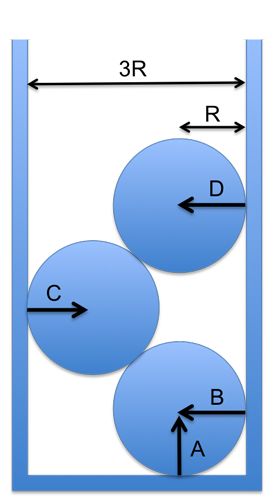
\includegraphics[scale=1.0]{Graphics/h9p7}
\end{center}

``Three smooth balls of iron of mass $m$ and radius $R$ are placed inside a tube of diameter $3 R$ (see Figure). Find the magnitude of the forces ($A$, $B$, $C$ and $D$) exerted by the sides of the container on each ball. Write your answers in terms of $m$, $g$ and $R$.''

I will begin by assuming that there is no friction. That means that forces D, C and B are purely horizontal, and that force A is purely vertical. It also means that the middle ball must provide both an upwards and a rightwards force on the top ball.

Drawing this out (anything else might just be insanity; see partial drawing below), it's clear that $A = 3 m g$, or there cannot be equilibrium, if it A is the only upwards force.

The distance between the center of the bottom ball and the center of the middle ball is exactly $2 R$ (same for the middle and top balls).\\
The distance from the right side to the center of the bottom ball is $R$; the distance from the left side to the center of the middle ball is also $R$. Therefore, since the entire tube is $3 R$, the horizontal distance between the two centers must also be $R$.

Using the Pythagorean theorem, the vertical distance between the centers must then be $\sqrt{3}$ times $R$ (for both the top-middle and the middle-bottom balls).

So, forces... forces...\\
Consider the forces on the top ball. There is a force to the left, which cannot cause a torque relative to its center, since the angle between the position vector and the force vector would be 180 degrees.\\
Likewise, $m g$ due to gravity cannot cause a torque, as it acts on the center.\\
This means that only the contact force due to the middle ball remains, which must therefore \emph{create no torque}, or the top ball would have a net torque! There is no other force that could possibly create an opposing torque and cancel it out.\\
The only way this can happen is if the net normal force is pointing straight towards the center of the top ball!

This then puts another constraint on the normal force, so we now know: it must be $D$ in magnitude to the right (or there is a net horizontal force on the top ball), $m g$ up (or there is a net downwards force on the top ball), \emph{and} be at the correct angle, or there is a net torque.

We can draw a triangle showing the angle; as mentioned, it is $R$ wide and $\sqrt{3} R$ high, with a $2 R$ hypotenuse (between the two balls' centers). Drawing the angle, we find

\begin{equation}
\tan \alpha = \frac{\sqrt{3}R}{R} = \sqrt{3}
\end{equation}

We then draw a vector triangle for the forces; the angle must be the same, or the net force won't point towards the center of the top ball! For the same $\alpha$, clearly $\tan \alpha$ must also be the same. Relating the forces instead, we have $D$ horizontally and $m g$ on the vertical side, so

\begin{equation}
\tan \alpha = \frac{m g}{D}
\end{equation}

\begin{center}
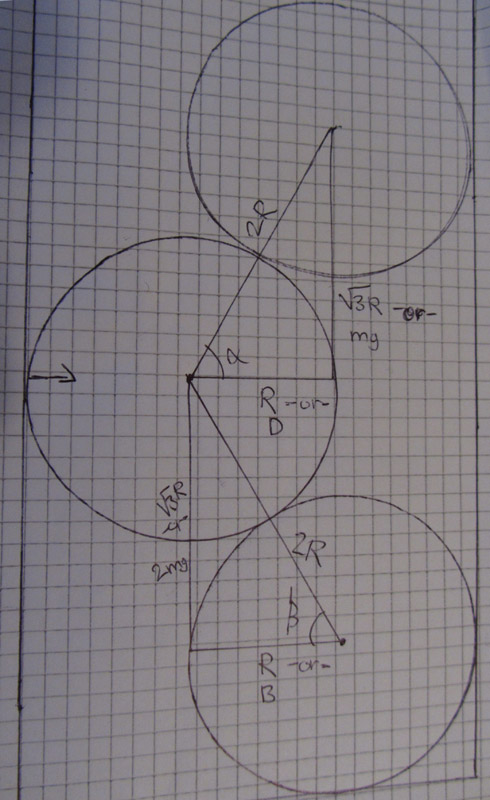
\includegraphics[scale=0.7]{Graphics/h9p7-sol}
\end{center}

I didn't label the forces here, since it make it very difficult to get it at all readable. Doing so is practically mandatory to solve this though, in my opinion; this was my second, simplified drawing.\\
(This is perhaps the cleanest thing I've drawn in years, which is why I don't post hand-drawn stuff often. It's usually much harder to read, which says something!)

$\alpha$ must then be the same for the net force vector, or that force will create a torque on the top ball. We can set the two tangents equal and find $D$:

\begin{align}
\frac{m g}{D} &= \sqrt{3}\\
D &= \frac{m g}{\sqrt{3}}
\end{align}

Nice! What about the bottom ball? We have a very similar situation there! There is an upwards force $2 m g$ to the middle ball instead of $m g$, since the bottom ball supports both of those above it.

For the sides, we again find:

\begin{equation}
\tan \beta = \frac{\sqrt{3} R}{R} = \sqrt{3}
\end{equation}

The forces again need the same angle, so we can find the tangent for the forces, and set the two equal again:

\begin{align}
\tan \beta &= \frac{2 m g}{B}\\
\sqrt{3} &= \frac{2 m g}{B}\\
B \sqrt{3} &= 2 m g\\
B &= \frac{2 m g}{\sqrt{3}}
\end{align}

Finally, for the middle ball, we can simply sum the horizontal forces; the one to the right needs to be equal to the sum of those to the right, or there is a net force. $C$ to the right must cancel with $B + D$ to the left, and we know those two.

\begin{align}
C &= B + D\\
C &= \frac{2 m g}{\sqrt{3}} + \frac{m g}{\sqrt{3}} = \frac{3 m g}{\sqrt{3}} = \frac{3 \sqrt{3} m g}{3} = \sqrt{3} m g
\end{align}

And that's it! Easy once I found the trick, but I have to admit it took a while. If I hadn't drawn it out, it would have been way harder.

\section{Problem 8: Two flywheels and a drive belt}

\begin{center}
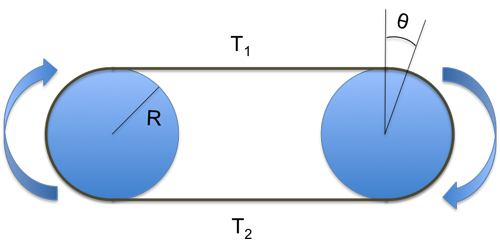
\includegraphics[scale=1.1]{Graphics/h9p8}
\end{center}

``The flywheel of a motor is connected to the flywheel of an electric generator by a drive belt. The flywheels are of equal size each of radius $R$. While the flywheels are rotating the tension in the upper and lower portions of the drive belt are $T_1$ and $T_2$ respectively. The drive belt exerts a torque $\tau = (T_2-T_1) R$ on the generator (around its center). The coefficient of static friction between the drive belt and each flywheel is $\mu_s$. Assume the tension is as high as possible with no slipping between the belt and the flywheel, and that the drive belt is massless.

(a) Derive a differential expression representing the change of tension along the portion of the belt in contact with one of the flywheels. That is find the value of $dT/T$ for one of the two flywheels. $dT/T = $''

\begin{enumerate}
\item $\displaystyle \frac{1}{\mu_s} d\theta$
\item $\displaystyle \frac{1}{\mu_s R} d\theta$
\item $\displaystyle \mu_s d\theta$
\item $\displaystyle R \mu_s d\theta$
\end{enumerate}

What is $T_1$?

\begin{enumerate}
\item $\displaystyle \frac{\tau}{R} \frac{1}{e^{\mu_s \pi} - 1}$
\item $\displaystyle \frac{\tau}{R} \frac{1}{1 - e^{-\mu_s \pi}}$
\item $\displaystyle \frac{\tau}{R} e^{\mu_s \pi}$
\item $\displaystyle \frac{\tau}{R} e^{-\mu_s \pi}$
\item $\displaystyle \frac{\tau}{R} (1 - e^{\mu_s \pi})$
\end{enumerate}

What is $T_2$?

\begin{enumerate}
\item $\displaystyle \frac{\tau}{R} \frac{1}{e^{\mu_s \pi} - 1}$
\item $\displaystyle \frac{\tau}{R} \frac{1}{1 - e^{-\mu_s \pi}}$
\item $\displaystyle \frac{\tau}{R} e^{\mu_s \pi}$
\item $\displaystyle \frac{\tau}{R} e^{-\mu_s \pi}$
\item $\displaystyle \frac{\tau}{R} (1 - e^{\mu_s \pi})$
\end{enumerate}

The equations look like capstan equations, which is not entirely unexpected: we have differing tensions in something wound around a cylinder (or two).\\
Indeed, the recommended reading is the book's derivation of the capstan equation.

Let's start by looking at part one. I will look at the rightmost wheel, and basically assume the other one doesn't exist.\\
$T_2 > T_1$, or the torque would be in the opposite direction of the rotation, and so it wouldn't be in any kind of equilibrium. Therefore, the frictional force is counterclockwise along the wheel, ``helping'' $T_1$, so that there can be equilibrium.\\
We therefore have the same situation as the book, and don't need to think of the opposite case (reversing directions or such).

Since the derivation is fairly complex, and the book derivation applies to this situation, I will use some results from there, to get started. There is a sign difference that we can ignore if we only keep track of directions/which tension is the larger one.

\begin{equation}
\frac{dT}{T} = \mu_s d \theta
\end{equation}

for one wheel, which answers part (a) as-is.\\
Part (b) is not as straightforward, with or without the book's help. First, we have one useful relationship given to us in the question:

\begin{equation}
\tau = R(T_2 - T_1) \Rightarrow \frac{\tau}{R} = T_2 - T_1
\end{equation}

We'll need that later.\\
If we integrate the previous equation, from $T_1$ to $T_2$ on the left-hand side, and from $0$ to $\pi$ on the right, we find

\begin{equation}
\ln\frac{T_2}{T_1} = \mu_s \pi \Rightarrow \frac{T_2}{T_1} = e^{\mu_s \pi}
\end{equation}

And so, indeed, $T_2$ will be larger than $T_1$. Solved for $T_2$, we have, of course

\begin{equation}
T_2 = T_1 e^{\mu_s \pi}
\end{equation}

We now have two equations and two unknowns, so we can solve the rest from here.

\begin{align}
\frac{\tau}{R} &= T_2 - T_1\\
T_2 &= T_1 e^{\mu_s \pi}
\end{align}

We can find $T_1$ by substitution; we stick $T_1 e^{...}$ in for $T_2$ in the first equation and solve:

\begin{align}
T_1 e^{\mu_s \pi} - T_1 &= \frac{\tau}{R}\\
T_1 \left(e^{\mu_s \pi} - 1\right) &= \frac{\tau}{R}\\
T_1 &= \frac{\tau}{R} \frac{1}{e^{\mu_s \pi} - 1}
\end{align}

We have a simple relationship between $T_2$ and $T_2$ above, so finding $T_2$ is trivial now -- at least getting it mathematically equivalent. To get it to look like one of the answer options (as this was the week's only multiple choice question), we need to divide through by the exponential, and use $1/e^{x} = e^{-x}$:

\begin{align}
T_2 = T_1 e^{\mu_s \pi} &= \frac{\tau}{R} \frac{e^{\mu_s \pi}}{e^{\mu_s \pi} - 1}\\
                        &= \frac{\tau}{R} \frac{1}{1 - \frac{1}{e^{\mu_s \pi}}}\\
                        &= \frac{\tau}{R} \frac{1}{1 - e^{-\mu_s \pi}}
\end{align}

\section{Problem 9: Hanging rod length}

``A long rod hangs straight down from one end. How long (in meters) can the rod be before its weight causes it to break off at the end if it is made of iron? Titanium? Give your answer in meters.

Use the following values for densities and tensile strengths:

The densities of iron and titanium are $\SI{7.8e3}{kg/m^3}$ and $\SI{4.5e3}{kg/m^3}$ respectively.

The breaking - ultimate tensile strength: 350 MPa for iron and 450 MPa for titanium (MPa = $10^6 \text{ N/m}^2$).''

Hmm, I wonder if this can be solved in the very naive way. If we consider it attached at the very top, then essentially 100\% of the weight is below that point. Therefore, we only need to find the stress due to the weight of the entire bar, $m g = (A L \rho) g$.

The ultimate tensile stress is given as a pressure, force per unit area; $P_{ult} = F/A$. We need to multiply it by the cross-sectional area $A$ to find a force (comparable to a weight, since both are in newtons):

\begin{equation}
A L \rho g = P_{ult} A
\end{equation}

$A$ cancels:

\begin{align}
L \rho g &= P_{ult}\\
L &= \frac{P_{ult}}{\rho g}
\end{align}

And indeed, plugging in the values, this is correct! The answers are 4574 m (4.6 km) for iron, and 10194 m (10.2 km) for titanium.

\end{document}